\scanpage{366}
\mspage{5}
\uline{Dem 1)}\quad Seminaire Cartan

On regarde la suite spectrale du classifiant
\[
E_2\simeq\operatorname{Tor}^{H_*(K(\mathbb F_p,n),\mathbb F_p)}(\mathbb F_p,\mathbb F_p)
\Longrightarrow H_*(\underbrace{K(\mathbb F_p,n+1),\mathbb F_p}_{\substack{\rotatebox{90}{$=$}\\\mathord{\begin{tikzpicture}[baseline=(B.base)]\node[draw,ellipse,inner sep=2pt] (B) {$B_{K(\mathbb F_p,n)}$};\end{tikzpicture}}}}]
\]
Suite sp d'Eilenberg - Moore

Steenrod - Rothenberger, etc --
\figure{\begin{tikzpicture}
\draw (0,.8)--(.15,.82);\draw (.35,.75)--(.8,.76);\draw (1.05,.72)--(1.5,.7);\draw (1.5,.7)--(1.58,.59);\draw (1.85,.65)--(2,.65);\draw (2.45,.52)--(2.5,.54);
\draw (-.4,-.5)--(0,-.1)--(.1,-.14)--(1.1,-.02);\draw (2.1,.02) .. controls (2.35,.02) and (2.4,-.08) .. (2.5,-.08);
\end{tikzpicture}}
\diagram{\begin{tikzcd}[column sep=small]
\underline{Z(G\times G)}&\mathord{\begin{tikzpicture}[baseline=(ZG.base)]\node[draw,ellipse,inner sep=2pt] (ZG) {$ZG$};\draw (ZG.center) ellipse (0.45 and 0.30);\draw (ZG.center) ellipse (0.52 and 0.37);\end{tikzpicture}}\arrow[r]&\mathbb Z\\
ZG\otimes ZG\arrow[ur,shift left=3]\arrow[ur]\arrow[ur,shift right=3]&&{}
\end{tikzcd}}
\deleted{$\otimes ZK(\mathbb F_p,n)$}
\diagram{\begin{tikzcd}[column sep=small]
&&N\mathord{\begin{tikzpicture}[baseline=(ZK.base)]\node[draw,ellipse,inner sep=2pt] (ZK) {$\underline{\underline{ZK(\mathbb F_p,n)}}$};\end{tikzpicture}}&\simeq M\\
&&\text{alg diff graduée}&{}\\
&&\text{Bar Constr}\quad\text{augmentée.}\arrow[d,no head]&{}\\
\deleted{\otimes}H_*(K(\mathbb F_p,n)^{\otimes2}\arrow[r,shift left=3]\arrow[r]\arrow[r,shift right=3]&H_*K(\mathbb F_p,n)\arrow[r]&M_\bullet&{}
\end{tikzcd}}
\figure{
\begin{tikzpicture}\draw (0,0) .. controls (.8,.03) and (1.2,.06) .. (1.5,-.02);\end{tikzpicture}}
\[
A=Z(G)\qquad Z(EG)=*
\]
\diagram{\begin{tikzcd}[execute at end picture={\draw (0,0) ellipse (.7 and .3);\draw (0,0) ellipse (.8 and .35);}]
Z(BG)
\end{tikzcd}}
\figure{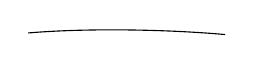
\begin{tikzpicture}\draw (0,0) .. controls (.7,.06) and (1.7,.05) .. (2.5,-.02);\end{tikzpicture}}

2) Methode de Serre\qquad Comm Helv\qquad1954
\margin{Springer:\par Symposium en l'honneur de Steenrod\par\uline{Article de}\par May.}
\[
H^*(K(\mathbb F,n+1,)\mathbb F_p)\otimes\underline{H^*(K(\mathbb F_p,n),\mathbb F_p)}\Longrightarrow\underline{H^*(*)}
\]
\figure{\begin{tikzpicture}\draw (0,.35) .. controls (-.35,.7) and (-.55,-.2) .. (0,-.3) .. controls (2,-.7) and (4,-.4) .. (4.5,-.1);\fill (.65,-.3) circle (.015);\fill (.8,-.4) circle (.015);\end{tikzpicture}}
\mspage{367}
